\chapter{Introduction}
\label{chap:introduction}
\begin{figure}[t]
    \centering
    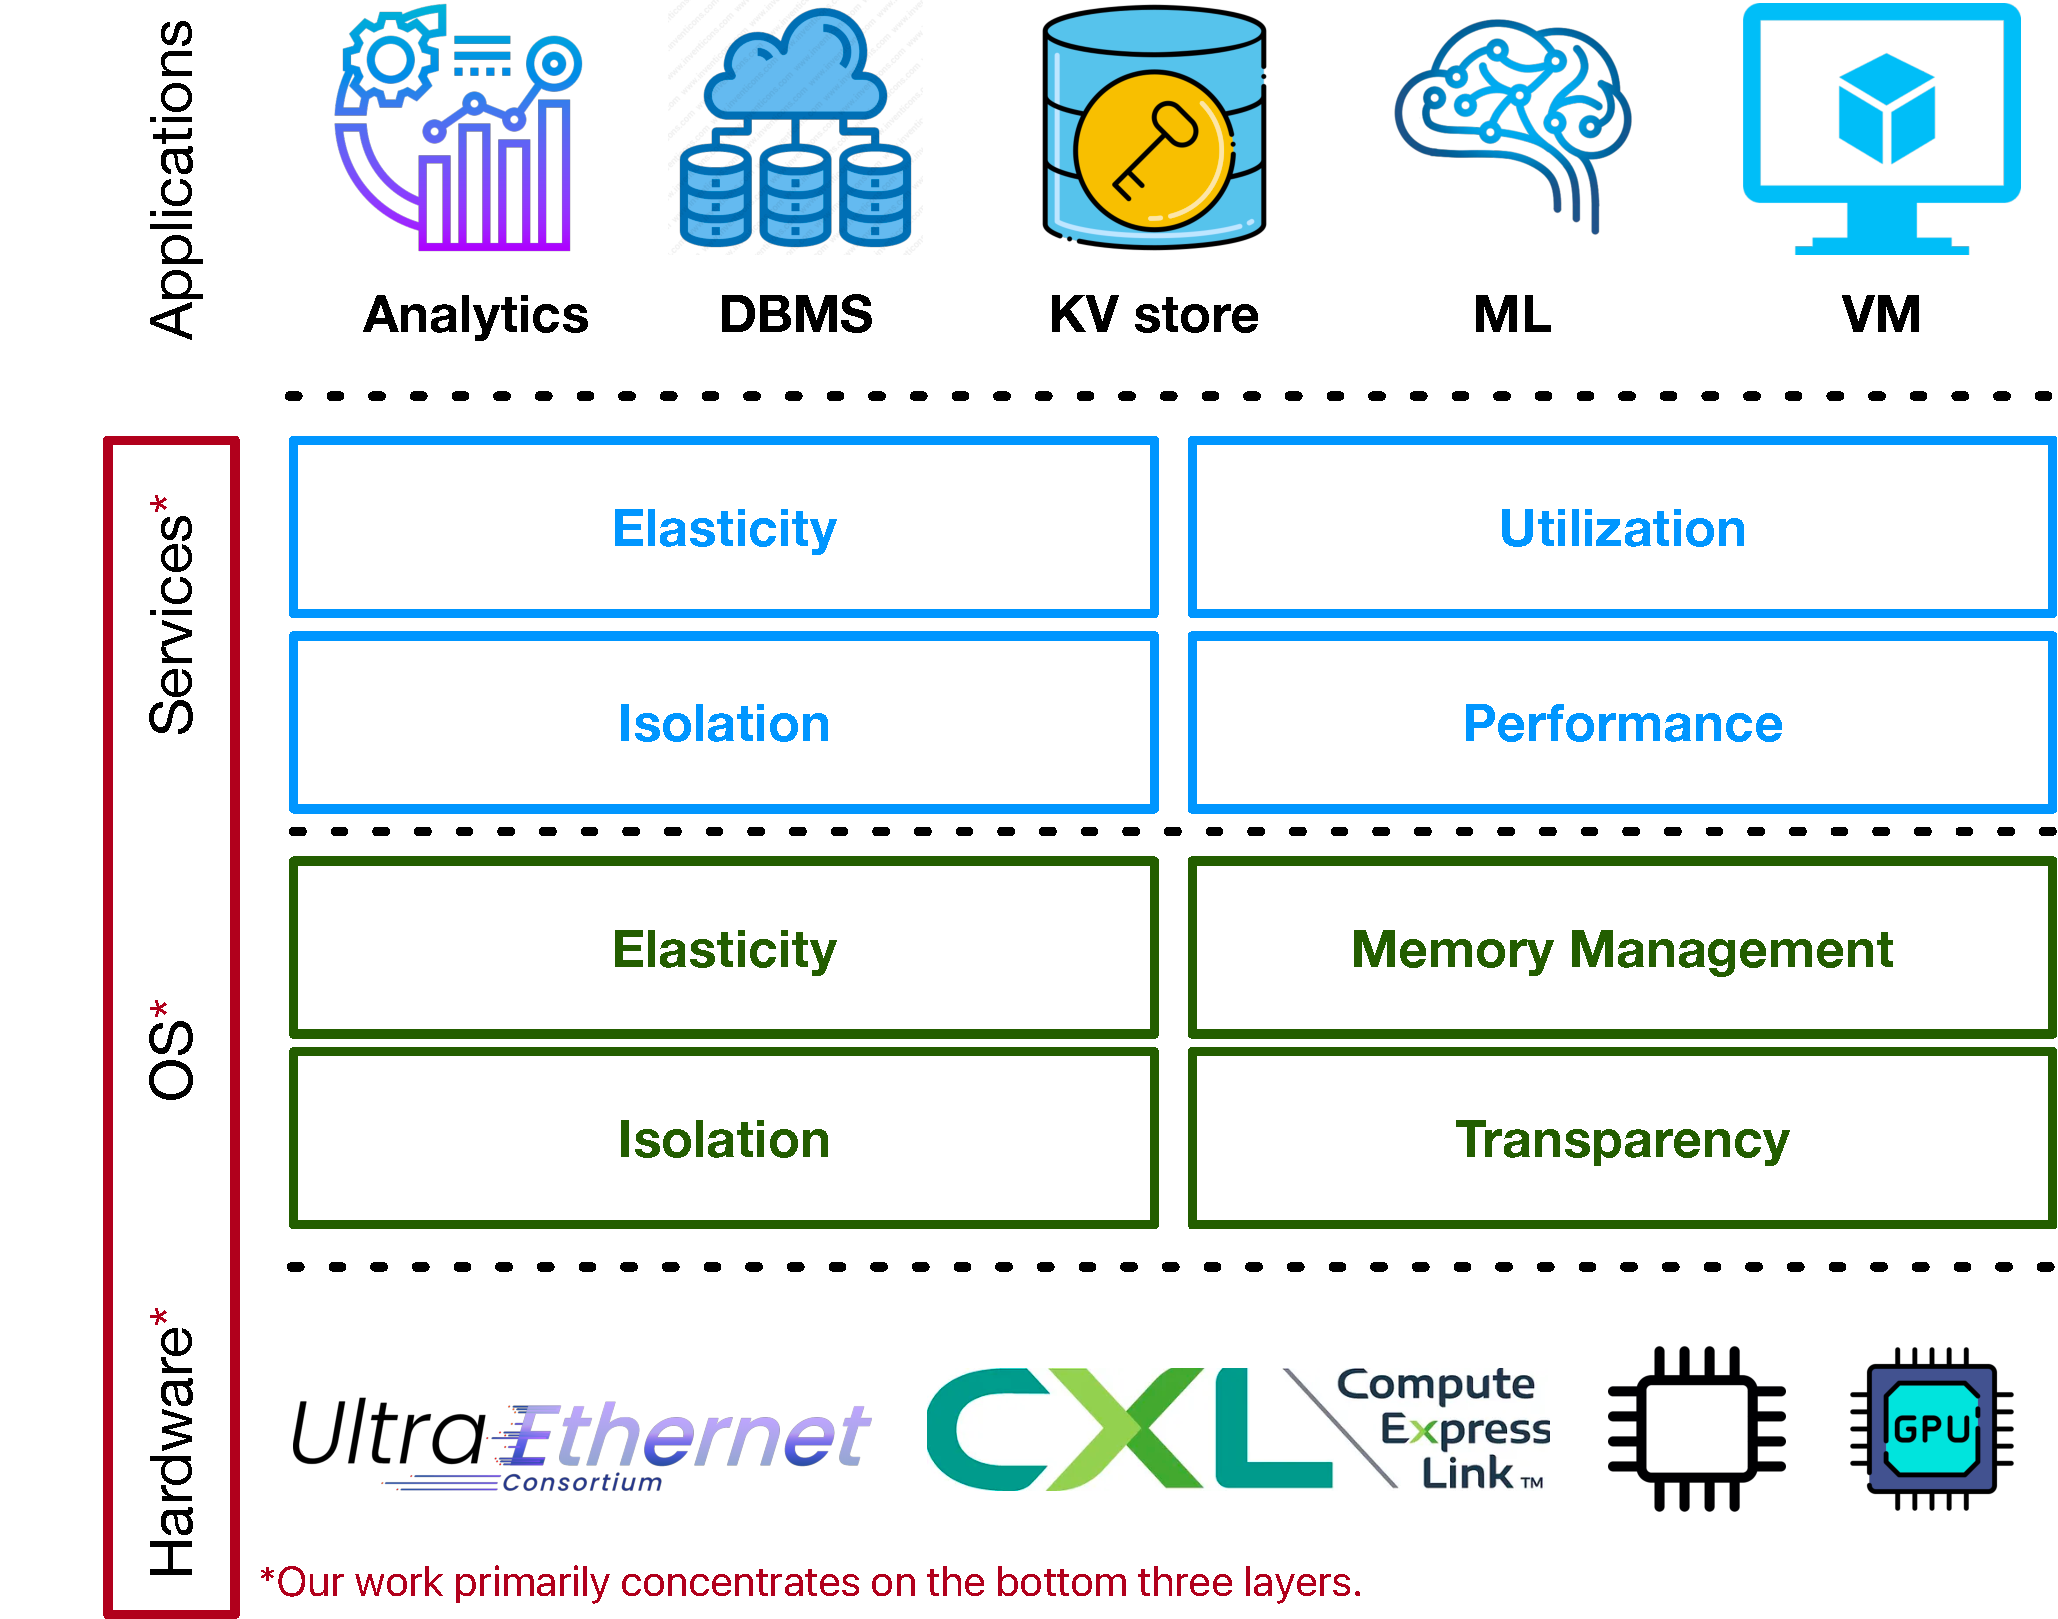
\includegraphics[width=0.8\columnwidth]{stack.pdf}
      \caption{\textbf{Cloud Stack of Disaggregated Architecture.}} \vspace{-1.0em}
      \label{fig:stack}
\end{figure}
The growing demand for scalable and efficient data center architectures has led to the emergence of resource disaggregation~\cite{mind, legoos, disagg, memdisagg1, memdisagg2, memdisagg3, memdisagg4, memdisagg5, memdisagg6}. This modern paradigm represents a significant shift from traditional monolithic server architectures. In conventional setups, servers are typically equipped with a fixed combination of compute, memory, and storage resources. In contrast, resource-disaggregated systems physically separate these resources and distribute them across various interconnects, such as networks~\cite{disagg, legoos, mind}, CXL~\cite{cxl, cxlasic}, and others. This separation allows for more flexible resource allocation and utilization.

Within the broader context of resource disaggregation in modern data center architectures, memory disaggregation~\cite{memdisagg1, memdisagg2, memdisagg3, memdisagg4, memdisagg5, memdisagg6} plays a crucial and foundational role. In traditional monolithic server configurations, memory often becomes a bottleneck, limiting the scalability and adaptability of applications. This issue has been frequently observed and reported in production data centers~\cite{memory1, memory2, memory3, memory4, memory5, memory6, memory7, memory8, memory9, memory10}. By decoupling memory resources from compute and storage elements and presenting them as pooled, disaggregated resources~\cite{pool1, pool2}, data centers can achieve increased efficiency, scalability, and adaptability. Memory-intensive applications~\cite{redis, ramcloud, sparkmemory} can access the memory they need on demand, without being constrained by the limitations of individual servers.

Memory disaggregation is the first step toward realizing the full potential of resource disaggregation, enabling data centers to efficiently allocate and utilize resources based on dynamic application needs. This ultimately leads to improved performance and better resource utilization.


\section{Limitations of Existing Approaches}

While resource disaggregation offers numerous advantages, transitioning existing applications to a disaggregated architecture is far from straightforward. Recent research has explored various approaches to address this challenge. Some efforts focus on adapting applications to optimize their use of disaggregated memory~\cite{farm, aifm, sherman, existing1}, while others aim to transparently port applications, shifting the responsibility of mitigating performance penalties—arising from the mismatch between disaggregated architectures and traditional software interfaces—to the service or operating system layer~\cite{mind, legoos, fastswap, infiniswap, runtime1, runtime2}.


The core issue lies in the fundamental mismatch between the existing cloud stack, designed for monolithic architectures, and the requirements of disaggregated architectures (Figure \ref{fig:stack}). The current cloud and hardware stacks are not inherently aware of the unique characteristics of disaggregated memory, leading to distinct challenges across different layers of the stack:

\paragraphb{Application interface} In disaggregated architectures, applications face unique challenges compared to traditional monolithic systems. The primary difference is resource distribution: compute, memory, and storage are spread across multiple nodes instead of centralized in one server. This requires complex communication and data management strategies to handle increased latency and resource management needs. In contrast, monolithic architectures offer integrated resources, simplifying application interaction. Adapting to disaggregated systems involves significantly redesigning applications for effective resource utilization and management.

\paragraphb{OS support} Unlike monolithic servers where the OS manages resources within a single server, the placement and function of the OS in disaggregated architectures are still subjects of debate in both industry and academia. Options include centralizing the OS at a single point~\cite{mind} in the architecture or disaggregating its functions across different resource nodes~\cite{legoos}.

\paragraphb{Performance overheads of disaggregation} Transitioning existing applications to a disaggregated architecture transparently introduces a spectrum of performance challenges. These include, but are not limited to, managing memory partitioning~\cite{jiffy} and addressing applications with irregular memory access patterns~\cite{chase}. Various other issues, such as latency sensitivity, bandwidth limitations, and the overhead of remote resource management, compound this complexity. These factors contribute to the overall performance penalty that disaggregated systems must carefully consider and mitigate.

\paragraphb{Future interconnects} Using networks as interconnects for resource disaggregation has been a subject of exploration in academia and industry. However, networks have inherent challenges, such as performance slowdowns compared to intra-server resource access and a lack of inherent coherency. Advanced hardware technologies like Compute Express Link (CXL)~\cite{cxl, cxlasic, pond} offer promising enhancements with faster access times and hardware-supported cache coherence. Yet, the current state of hardware prototypes and software support for these technologies remains limited.

\section{Thesis Overview}

In this dissertation, we attempt to take a top-down approach and explore the optimal memory management solutions for three most significant layers, i.e. Service, OS and Hardware layers of disaggregated memory architectures.

\subsection{Memory management as a Service}
With least modification to lower layers such as OS/Hardware, we explore the design requirement and challenges in provoding memory management as a service. We proposed an end-to-end system design called Jiffy, which enables multiple application/tasks multiplex memory in a elastic manner. Jiffy also provides multiple popular data structure interface and can be easily applied to existing cloud applications.
\subsection{In-network memory management OS-design}
As we decouple compute and memory resources in disaggregated architecture. There is no single host as if in monolithic architecture in order to implement the key unit of resource management - the operating system. We proposal a new generation operating system design by placing OS functionality inside the interconnects. We start by a system called MIND, addressing the basic problems in memory management, such as memory address translation, memory protection, and cache coherence between multiple hosts. Such resource decoupling and in-network memory management serves well for cache-friendly workload, but performs poor for cache-friendly workload due to the back-and-forth communication over the slower interconnects. We then develop optimizations for dealing with cache-unfriendly workloads. We design and implement a near memory accelerator from scratch, named PULSE. PULSE analyzes popular pointer traversal applications and identify a common but simple interface that can be easily integrated into existing cloud applications.
\subsection{Memory management adaptation for new-generation interconnects}
In prior work~\cite{mind,legoos}, ethernet is considered as the most popular interconnect for disaggregated data centers. However, as new memory interconnects are emerging, such as Compute Express Link(CXL), new adaptation of memory management needs to be made regarding the new interconnect interface. Within the context of disaggregated architecture, new problems arises such as how can the applications leverage multiple tiers of memory. Therefore, we start with a perfomance analysis on CXL 1.1 single host extended memory, and then we propose a new system design that integrates disaggregated CXL memory pool with today's emerging popular application - LLM inference.

\section{Outline and Previously Published Work}

This dissertation is organized as follows. Chapter~\ref{chap:service} introduces Jiffy, a distributed memory management system that decouples memory capacity and lifetime from compute in the serverless paradigm. Chapter~\ref{chap:os} describes two innovated system design: (1) MIND, a rack-scale memory disaggregation system that uses programmable switches to embed memory management logic in
the network fabric. (2) PULSE, a framework centered on enhancing in-network optimizations for
irregular memory accesses within disaggregated data centers. Chapter ~\ref{chap:hardware} presents our exploration in latest Compute Express Link(CXL) hardware. We conclude with our contributions and possible future work directions in Chapter~\ref{chap:future}.

Chapter~\ref{chap:service} revises material from~\cite{jiffy}\footnote{Work done in collaboration with Rachit Agarwal, Aditya Akella, and Ion Stoica}. Chapter~\ref{chap:os} revises material from~\cite{mind}\footnote{Work done in collaboration with Seung-seob Lee, Yanpeng Yu, Lin Zhong and Abhishek Bhattacharjee} and~\cite{chase}\footnote{Work done in collaboration with Seung-seob Lee and Abhishek Bhattacharjee}. Finally, Chapter~\ref{chap:hardware} revises material from~\cite{cxleurosys}\footnote{Work done in collaboration with the Bytedance Infrastructure team}.
